\section{Industrial context}

Dispersed two-phase flows play a critical role in numerous natural phenomena and industrial applications, making their accurate modeling an essential area of study.
These flows involve the interaction of a dispersed phase, such as droplets, bubbles, or solid particles, with a continuous phase, typically a gas or a liquid. 
For example, in environmental science, aerosols and pollutants in the atmosphere involve tiny particles dispersed in the air. 
Microplastic rods or fibers, as pollutants in water, represent a dispersed solid phase in a liquid continuous phase. 
Sediment transport in rivers, rain, and snowflakes in air, are also examples of dispersed two-phase flow systems. 
In energy and chemical engineering, fluidized bed reactors involve solid particles suspended in a continuous phase (gas or liquid flow),  while boiling flows in the nuclear industry deal with vapor bubbles dispersed in water. 
In Biomedical sciences, the modeling of blood flow also requires the study of dispersed two-phase flows as red blood cells (dispersed phase) are suspended in plasma (continuous phase). 

In the industry, sedimentation of particles falling or rising under the action of gravity is an efficient way to separate solid particles or droplets from the surrounding fluid. 
The clarification of wastewater makes use of such physics, the particles or droplets rise due to buoyancy forces, afterward they are removed from the mixture.
Even though numerous experimental and theoretical studies have been conducted on this topic, models are still limited in accuracy
 \citep{paisant2014modelisation,gemello2018modelling}. 
Therefore, this PhD work focuses on the theoretical and numerical modeling of buoyancy-driven droplets suspensions,  within the broader context of dispersed two-phase flow modeling.  

Let us now take the example of two processes of interest for IFP Energies Nouvelles, highlighting their physical implications and key challenges.  


\subsection{Liquid-Liquid extraction}


% The first process is liquid-liquid extraction, specifically the ``agitated'' liquid-liquid extraction process. 

The liquid-liquid separation process is a unit operation during which one or more solutes are transferred from one liquid phase (diluent or dispersed phase) to another liquid phase (solvent or continuous phase).
The solvent and diluent phases are either immiscible or partially immiscible.
The separation efficiency relies on the difference in solubility of the solute between the two phases.
Typically, the solvent is an aqueous phase, often water, while the diluent is an organic phase, such as a non-polar solvent like ether or kerosene.
As phase transfer is proportional to the concentration of interfaces between phases, small droplets are initially desirable to maximize the interfacial concentration.
At the end of the process, separating the diluent and solvent phases becomes the priority, thus, coalescence between droplets is promoted to enhance phase separation.

Let us now focus specifically on the agitated counter-current liquid-liquid extraction process, as illustrated in \ref{fig:liq-liq}. 
The schematic in \ref{fig:liq-liq} (middle) depicts the operation of the process.
The first step involves injecting the continuous solvent phase from the top of the column, while the dispersed phase (i.e., the feed solution containing the solute) is introduced through the bottom inlet (see \ref{fig:liq-liq}). 
In addition to the buoyancy forces that naturally cause droplets to rise, an artificial downstream flow of the continuous phase is generated because the outlet for this phase is located at the bottom of the vessel. 
This design increases the relative velocity between the phases, thereby renewing the continuous phase more frequently, hence optimizing the transfer of species.
As the droplets, which are less dense than the solvent, rise due to buoyancy, they pass through agitators (represented by gray circles in \ref{fig:liq-liq} (middle)). 
The agitators create turbulence and shear forces that break the droplets into smaller droplets, also enhancing mass transfer efficiency between the two liquid phases. 
Finally, the processed continuous liquid exits at the bottom of the vessel, while the dispersed phase exits at the top after separation. 

As an illustration, \ref{fig:liq-liq} (left) shows a typical laboratory reproduction of the liquid-liquid separation process. 
Here, the different layers of agitators used to create dispersion are visible. 
Additionally, \ref{fig:liq-liq} (right) depicts a real-scale industrial process, which spans several meters in height, highlighting the significant scale difference between laboratory setups and industrial applications. 
\begin{figure}[h!]
    \centering
    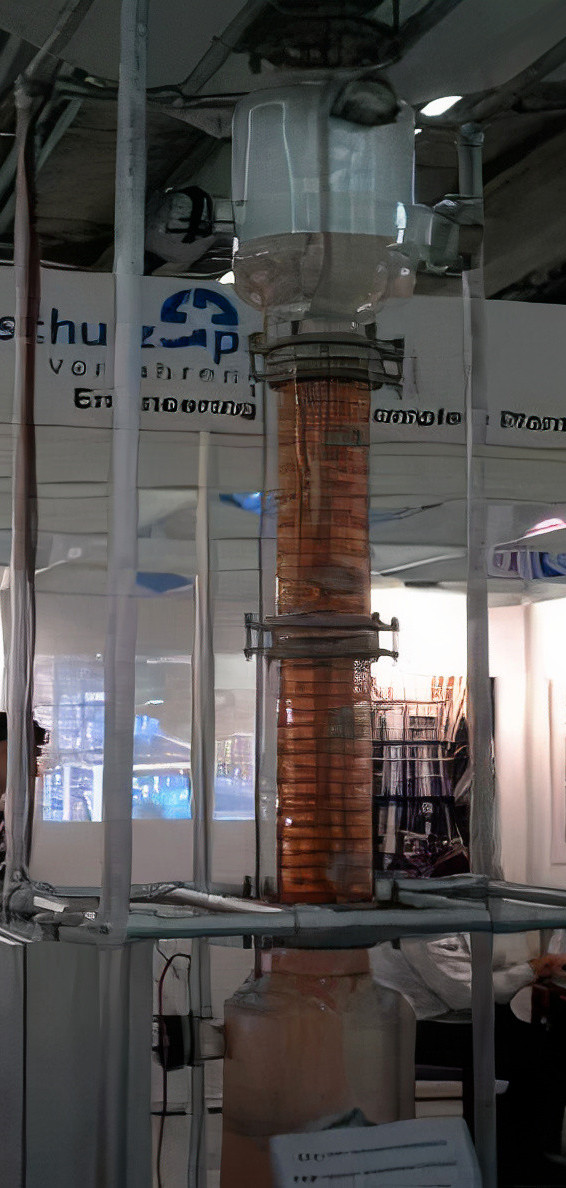
\includegraphics[height=0.3\textheight]{image/liq-liq_LE_auto_x5.jpg}
    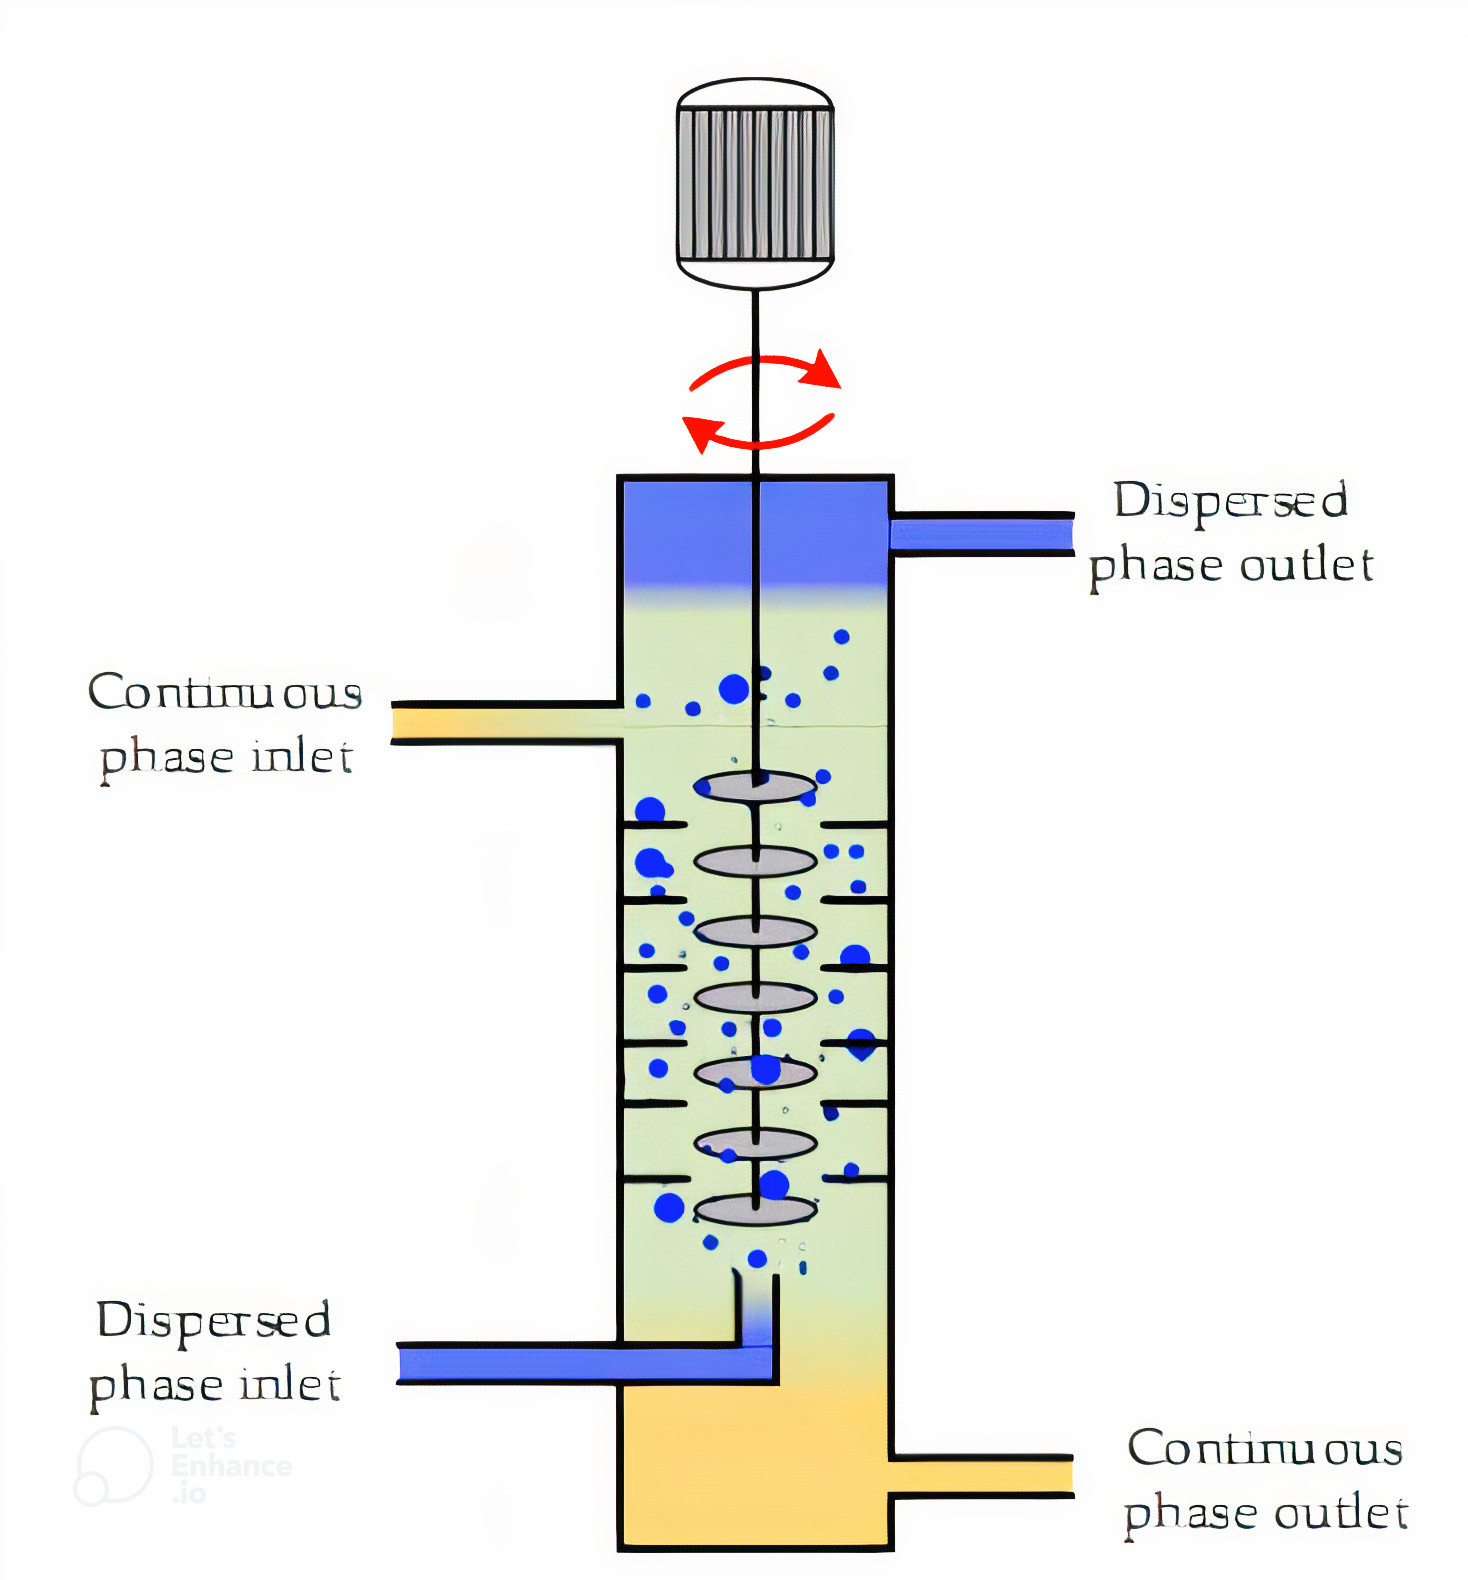
\includegraphics[height=0.3\textheight]{image/scheme_liq-liq_mieux.png}
    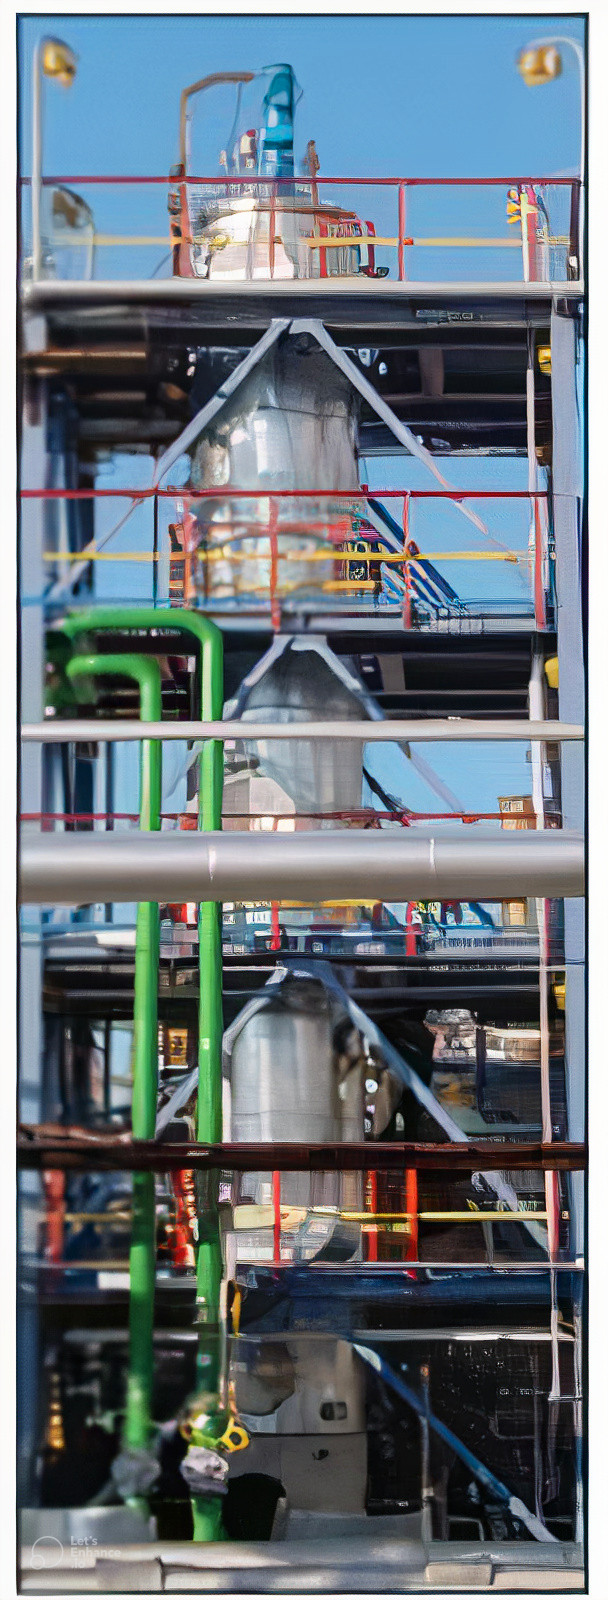
\includegraphics[height=0.3\textheight]{image/process_LE_auto_x4.jpg}

    % 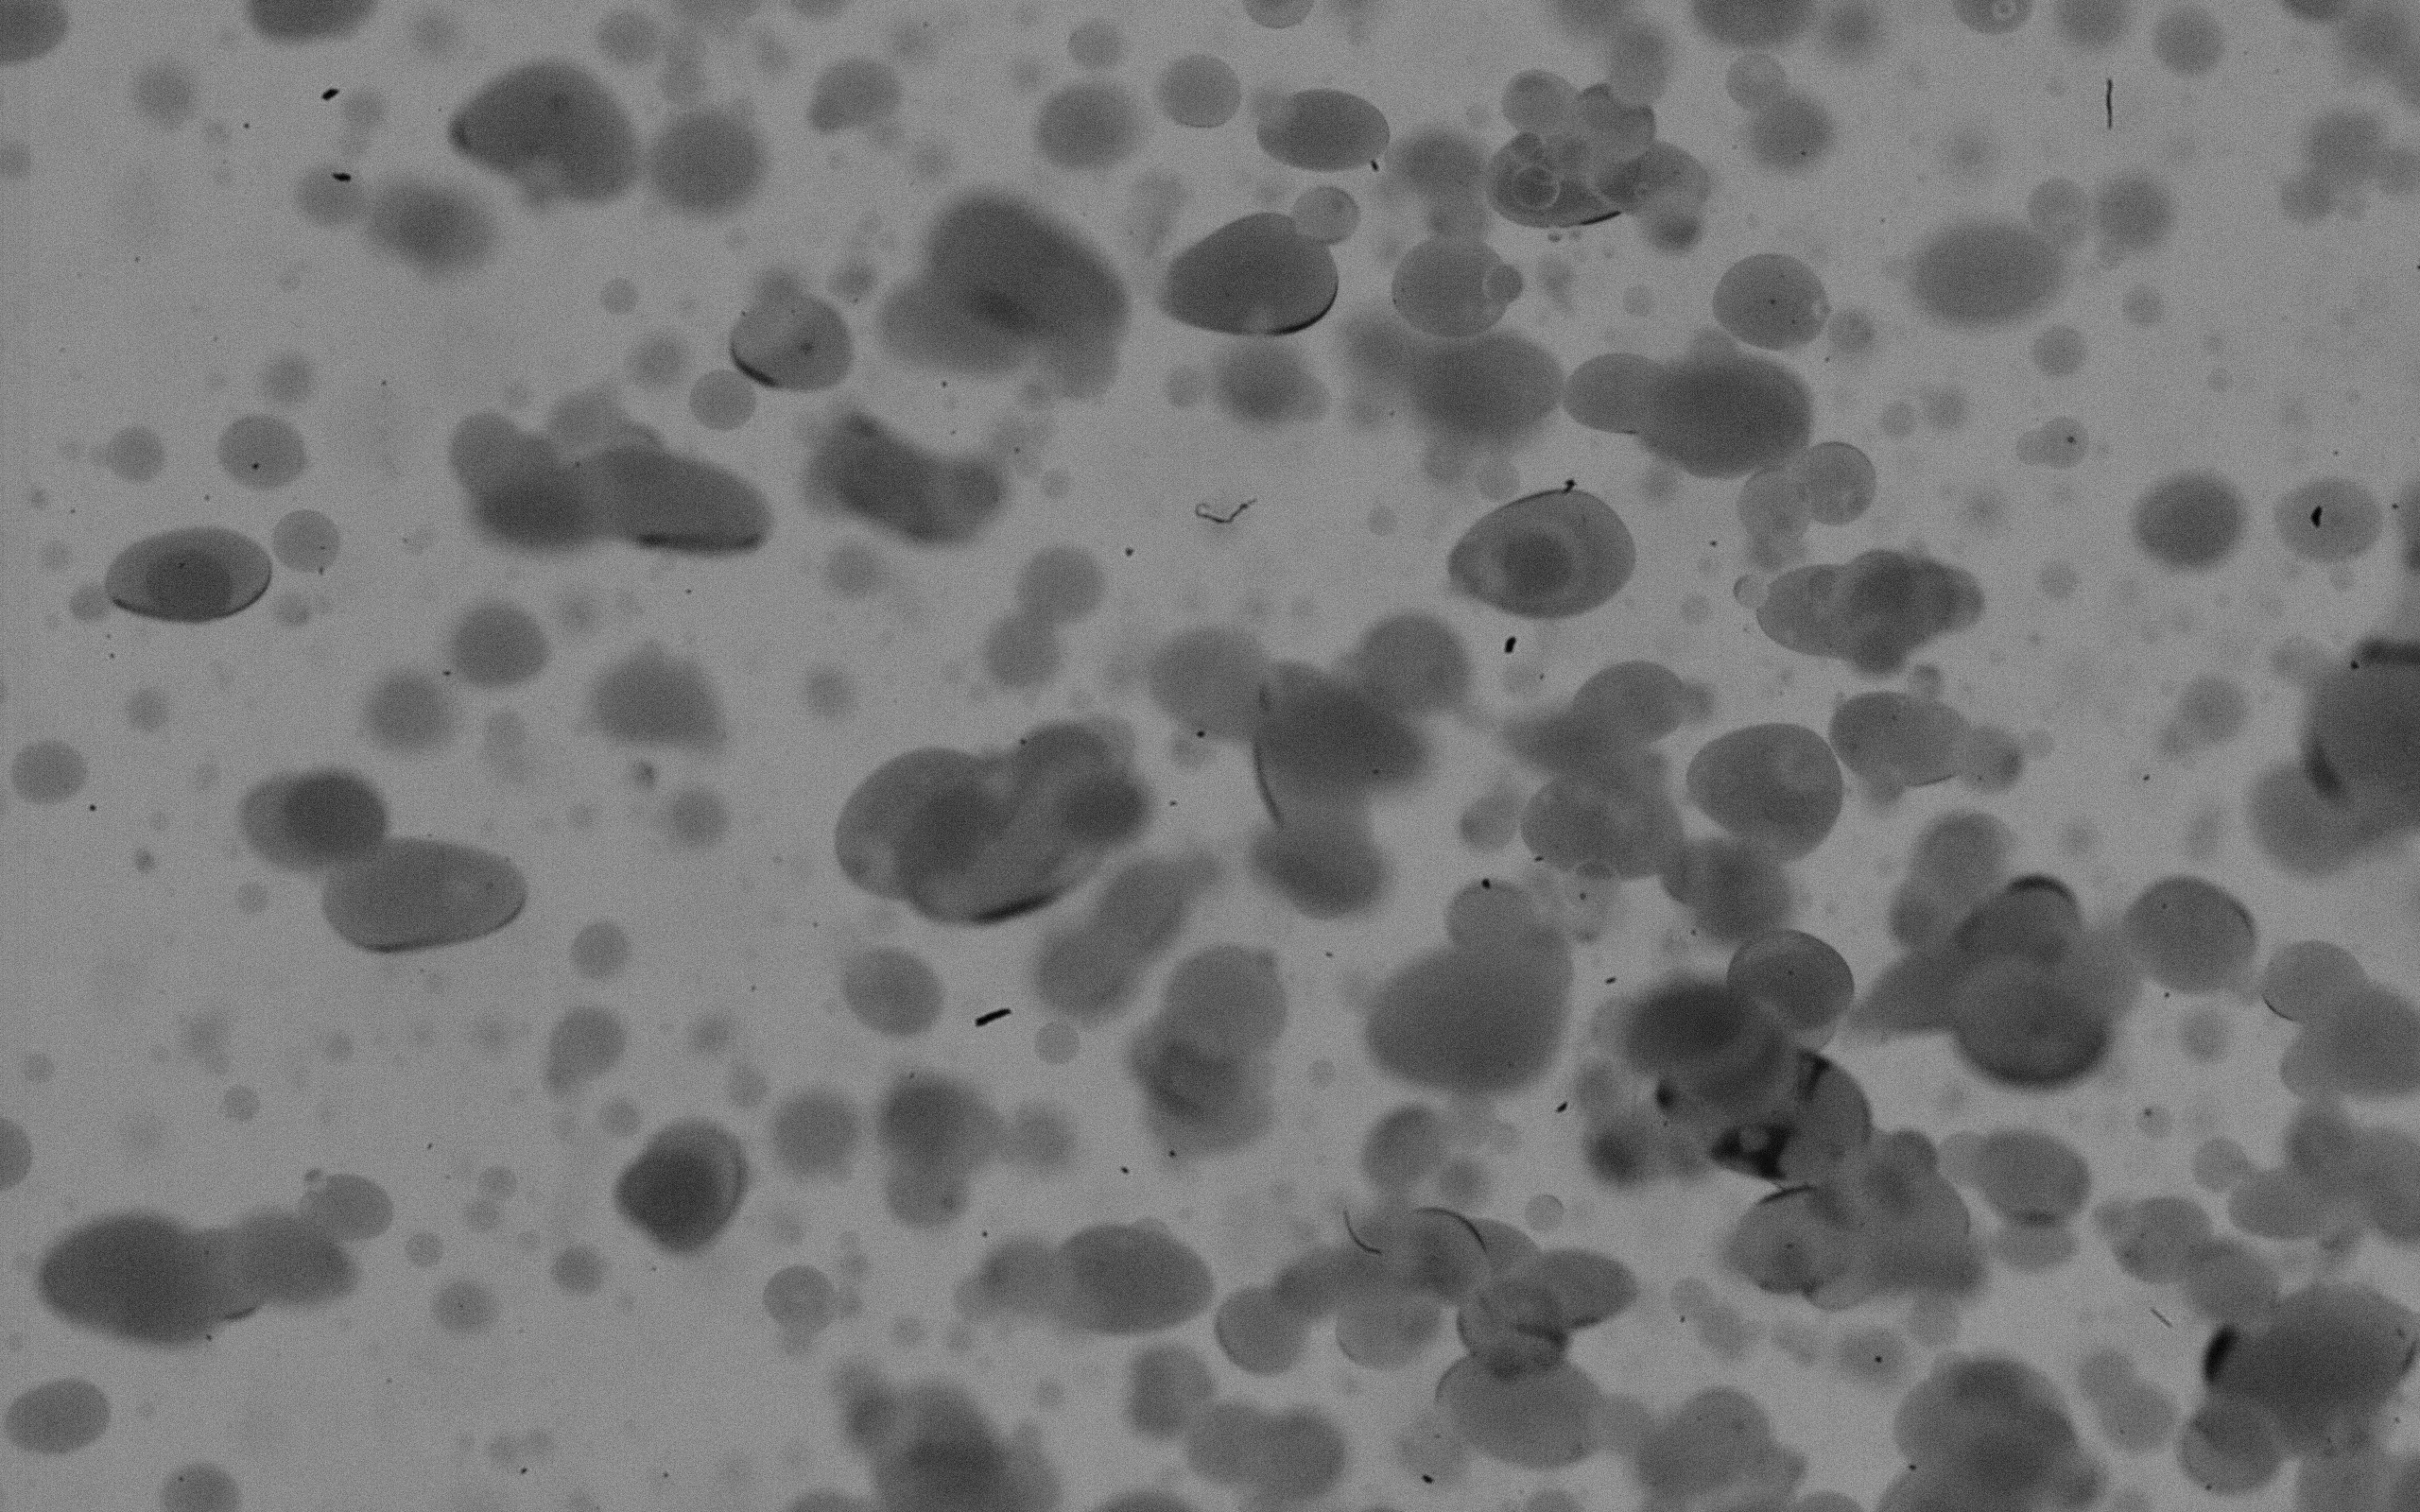
\includegraphics[height=0.15\textheight]{image/bubbles.png}
    \caption{
        (Left)   Pilot-scale illustration of the agitated liquid-liquid extraction process.
        (Middle) Schematic representation of the agitated liquid-liquid extraction process.
        (Right)  Industrial-scale liquid-liquid extraction process.
    }
    \label{fig:liq-liq}
\end{figure}



The aim of such a design is to transfer a species from one phase to another as efficiently as possible and subsequently to separate the diluent and solvent phases.
To achieve this, one must optimize the mass transfer rate between the phases based on hydrodynamic parameters, such as the operating conditions (e.g., input flow rates), the physical properties of the phases (e.g., density, viscosity, surface tension), and the geometry of the vessel and agitators.
Modeling such a process involves two major aspects.
(1) Thermodynamics modeling. This involves studying the migration of chemical species between the phases, including selecting suitable solvents and diluents to predict and optimize the separation efficiency of the mixture.
(2) Hydrodynamics modeling. This focuses on predicting the flow behavior of the continuous and dispersed phases within the vessel. Key considerations include determining the residence time of the droplets, their size distribution, and their relative velocity with respect to the solvent. These factors are crucial for accurately estimating the mass transfer rate within the vessel.



As this will be important for the following discussion, let us specify the typical length scales involved in these processes:
(1) Macroscopic length scale: This corresponds to the size of the vessel, typically on the order of several meters $\sim 10 \text{m}$, as illustrated in \ref{fig:liq-liq} (right). 
(2) Hydrodynamic or Mesoscopic length scale: This is determined by the typical size of a droplet of diluent, which is approximately $\sim 1 mm$. 
(3) Coalescence/breakup length scale: This is typically that of lubrication layers between droplets $\sim 1 \mu m$. 
(4) Nanoscopic length scale: If we examine the thermodynamic and chemical interactions occurring at the surface of the droplets, the relevant length scale is that of colloidal forces, which is approximately $\sim 1 nm$. 
As will be explained in more detail later, this extremely wide range of length scales makes the problem particularly challenging to analyze and model. 

To summarize, enhancing our understanding of the process requires characterizing and modeling the mass transfer in terms of both the local and global hydrodynamic properties of the flow within the vessel. 
This includes predicting the droplet velocity distributions and size distributions. 
Such models can be developed through small-scale experiments, such as those conducted in the pilot-scale column (\ref{fig:liq-liq} (left)) or through numerical simulations, as will be presented in the following. 
Once the underlying physics is fully understood and predictable, the process can be optimized effectively.


\subsection{Flotation process}

Over 80\% of the world’s wastewater is released into the environment without treatment \citep{ryder2017rapport}. 
This underscores the need to develop water treatment processes that are more efficient, compact, and energy-efficient. 
Among the various separation techniques employed in wastewater treatment, flotation represents a key method. 

The basic principle of flotation involves separating suspended inclusions in water, typically around $1\mu m$, by introducing air bubbles, approximately $\sim 1 mm$ in diameter, at the bottom of the vessel, see \ref{fig:flo} (left).   
As the bubbles ascend, they collide with the particles and eventually the particles get attached to the bubbles and rise with the bubble to the top of the vessel.
The waste particles, trapped within the foam formed by the bubbles at the surface, are then removed from the top of the vessel, leaving clear water behind.  
\begin{figure}[h!]
    \centering
    % 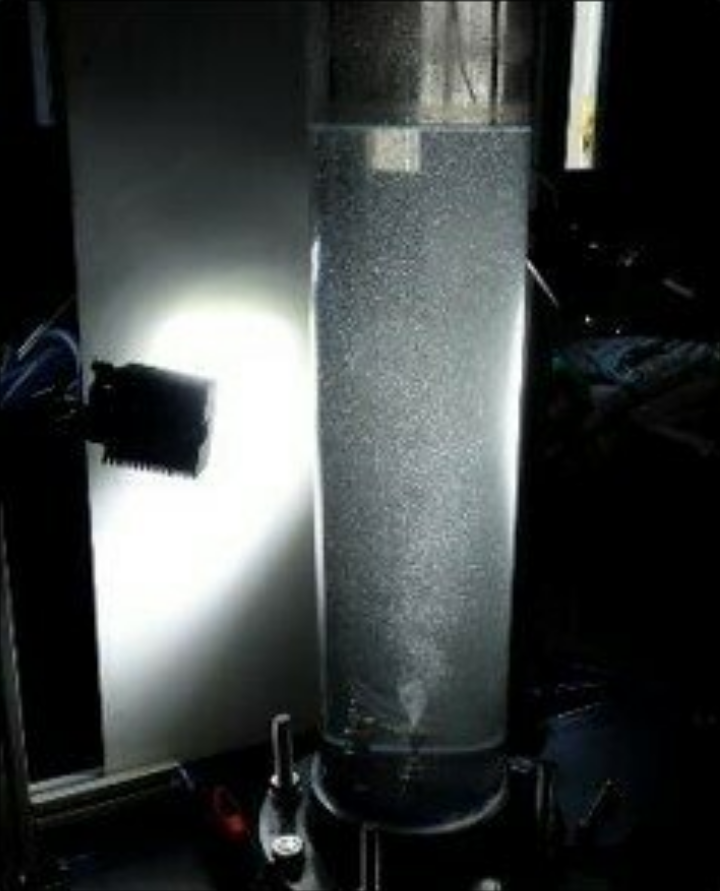
\includegraphics[height=0.3\textwidth]{image/flo.png}
    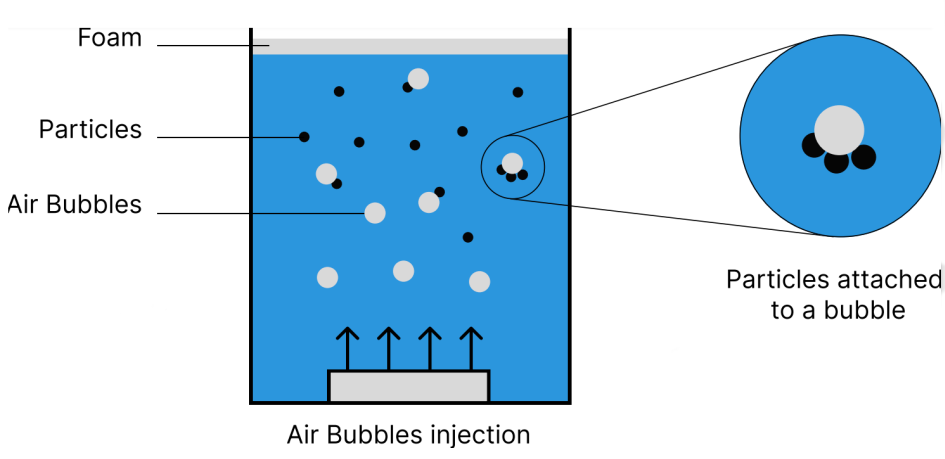
\includegraphics[height=0.3\textwidth]{image/flo_scheme.png}
    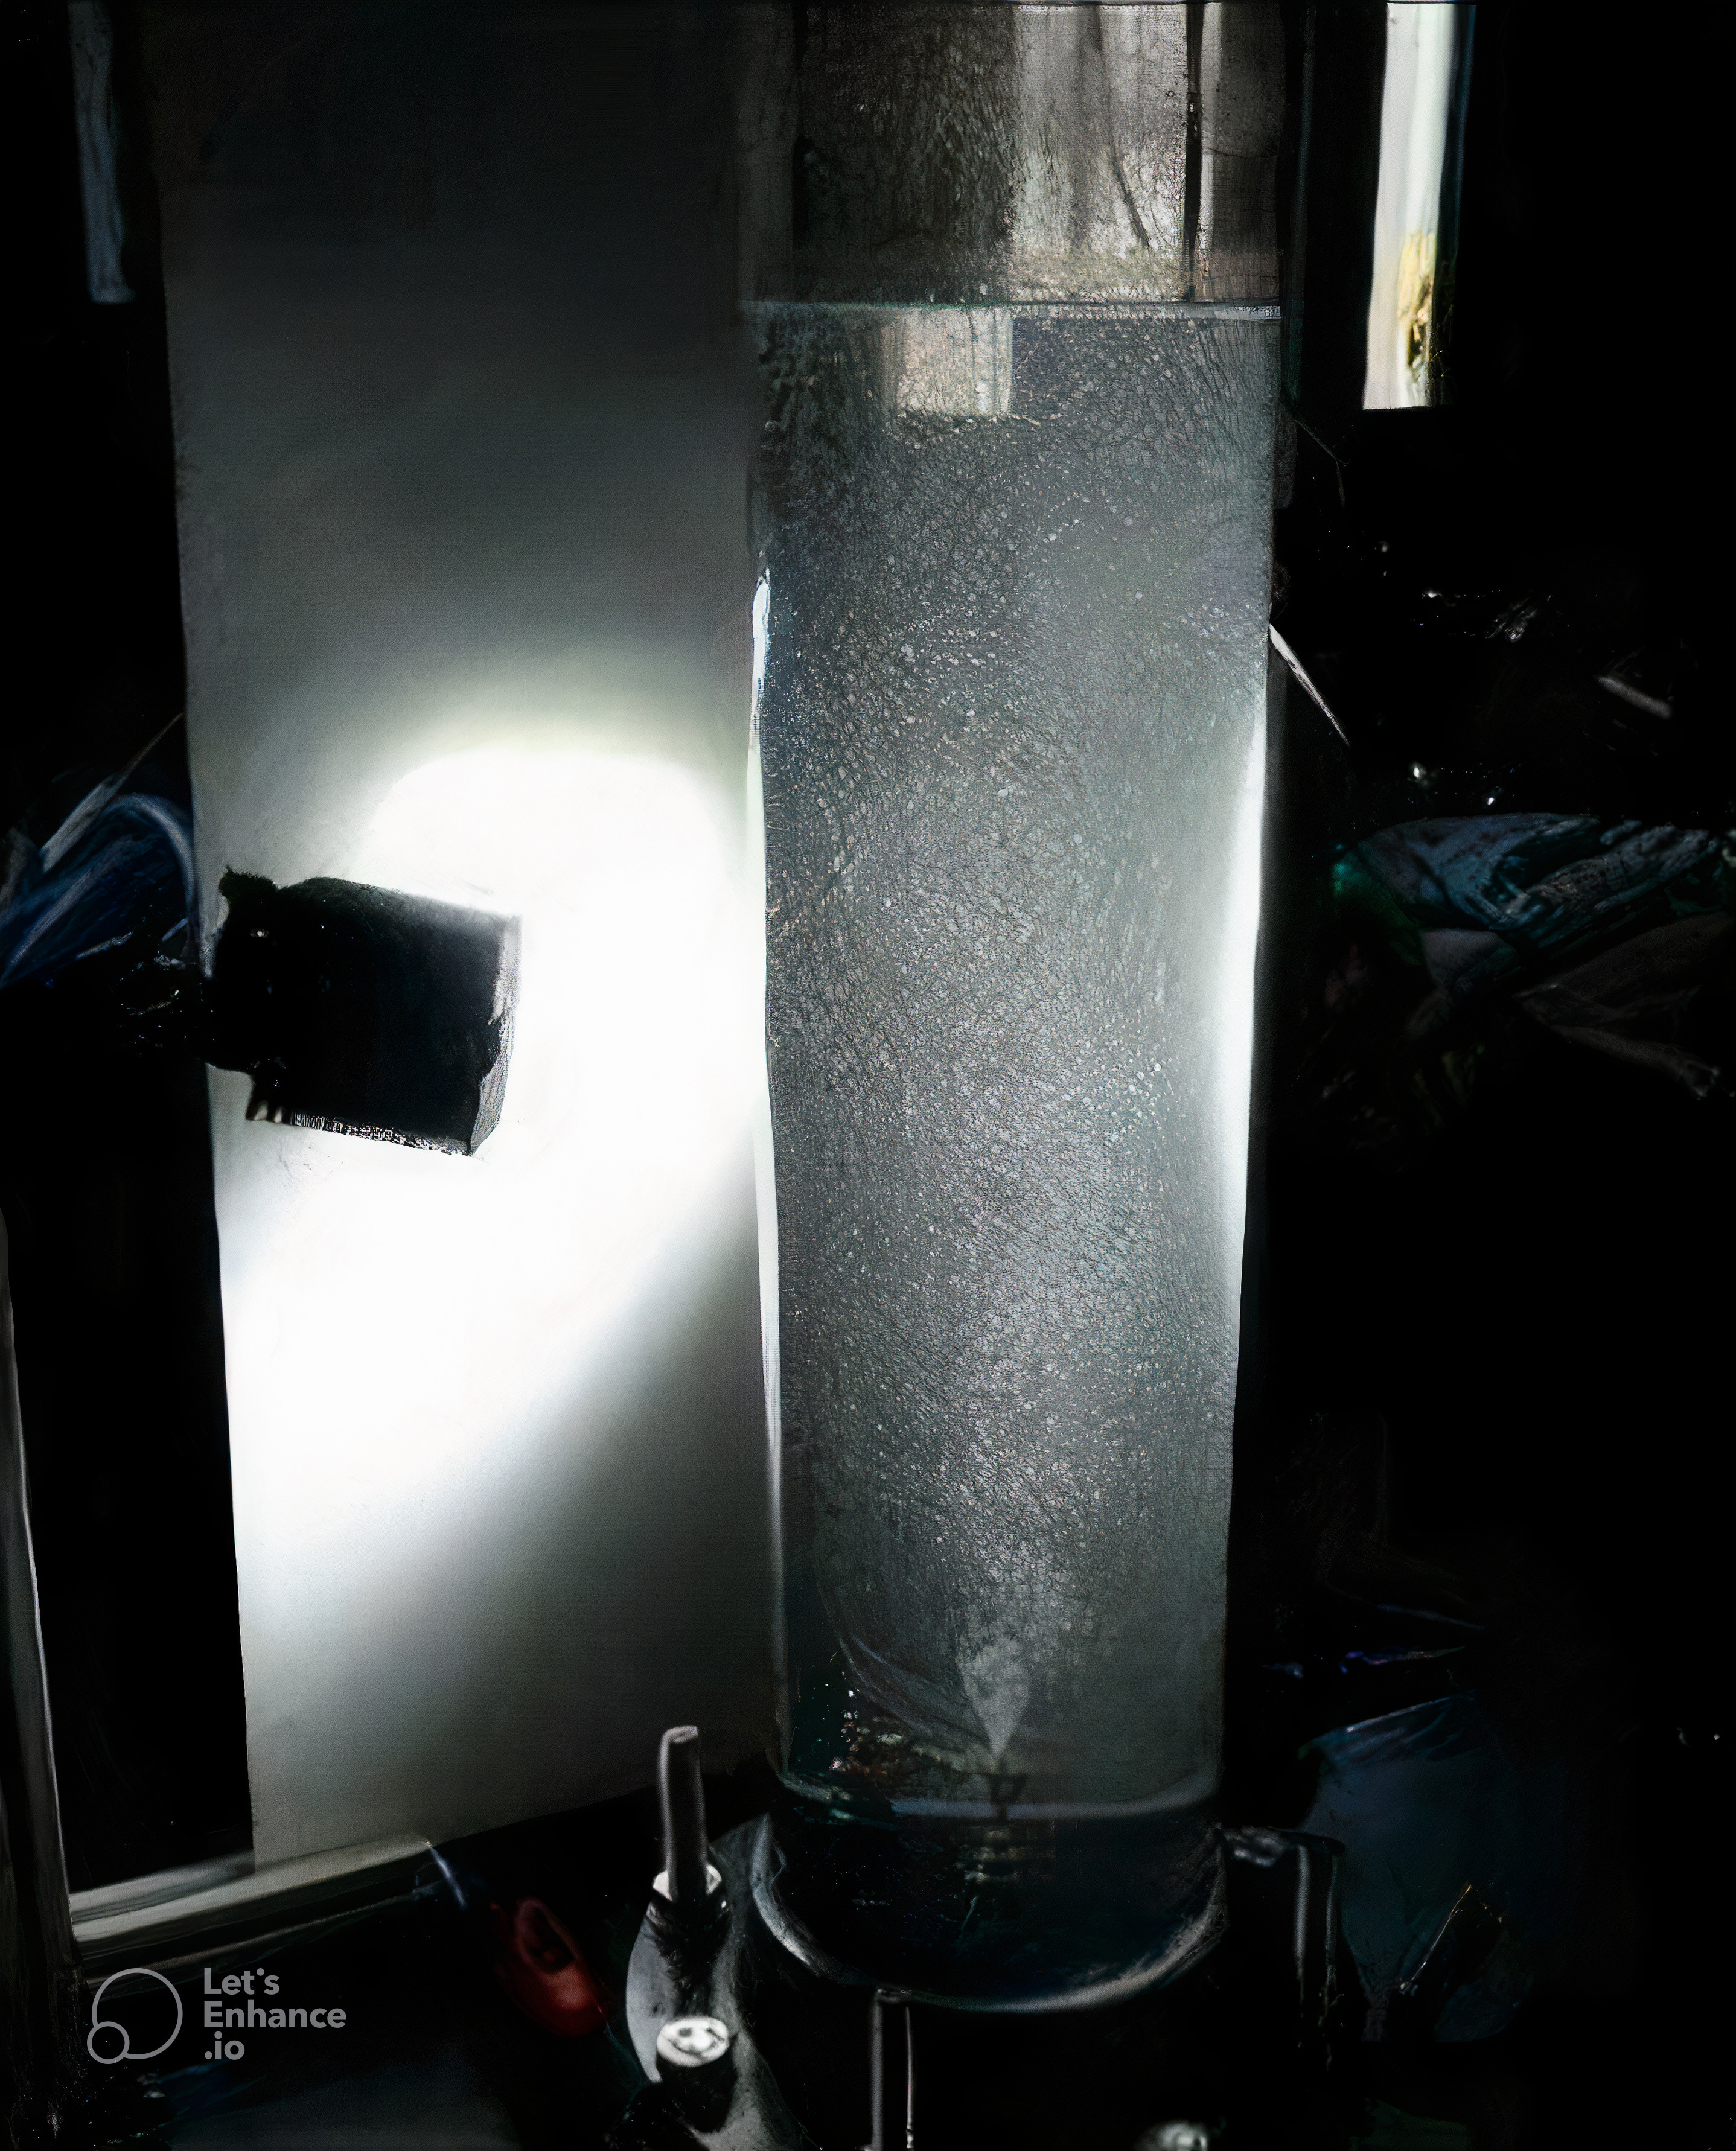
\includegraphics[height=0.3\textwidth]{image/flo_LE_auto_x4.jpg}
    \caption{
        (left) Scheme of the flotation column. 
        (right) Laboratory flotation column. 
        Reprinted from \citet{landal2025}.
        }
        \label{fig:flo}
\end{figure}

For illustrative purposes, we present in \ref{fig:flo} (right) a typical flotation column experiment. 
This design aims to optimize the rate at which particles (i.e., water waste) attach to bubbles and are subsequently removed from the continuous water phase. 
To achieve this, it is crucial to predict the global hydrodynamics, which includes the interactions between the dispersed and continuous phases, as well as particle-bubble and bubble-bubble interactions.
The bubble-particle interactions play a fundamental role, as they determine whether or not a particle attaches to the bubble. 
These interactions depend on various factors, such as the size and surface properties of both the particle and the bubble, their relative velocities, and the surrounding flow conditions. 
Thus, in this process, the size distribution of the dispersed phases and their velocities play an important role in determining the particle attachment rate to the bubbles.



To summarize, in order to model and optimize the flotation process, one must be able to accurately model the microscale interactions, such as the bubbles-particle interactions, across the entire vessel, which is typically on the order of several meters. 
Although the flotation process differs significantly from liquid-liquid separation, both processes share a common point: they involve modeling small bubbles, droplets, or solid particles immersed in a continuous phase that fills the vessel, with sizes on the order of $\sim 1000$ droplet-size. 
In this PhD work, we focus on modeling the interactions between droplets and the continuous phase, as well as between droplets themselves, while neglecting the interactions with smaller particles, for example. 
% The multi-scale nature of both the flotation and liquid-liquid extraction processes presents a major challenge in their modeling.



\section{A multiscale problem} 


As mentioned above the liquid-liquid multiphase flows, and more particularly, dispersed multiphase flows, often involve multiscale physical phenomena. 
Indeed, at the vessel scale, the liquid-liquid mixture can be approximated as two homogeneous phases, with effective properties that account for the droplet behavior in an averaged manner \citet{jackson2000}.
Then, the macroscopic properties and the hydrodynamics of the mixture depend on the microscale properties and the local interactions driving the physics at these scales. 

In the case of droplets, these interactions can be categorized into two types. The first type involves the hydrodynamic interactions between the dispersed phase and the continuous phase. 
The scale of interest here is the droplet scale, which is also referred to as the mesoscale. 
The second type of interaction arises from colloidal forces, which act at the molecular scale.
Indeed, when droplets come into contact, the thin fluid film separating them is sufficiently thin so that microscale forces, such as colloidal interactions, become non-negligible. 
Notably, the probability of two droplets coalescing upon contact is affected by these colloidal interactions. 
As a result, these interactions impact the droplet size distribution, influencing behaviors at the droplet scale, which in turn affect mass transfer and attachment probabilities in processes such as liquid-liquid extraction and flotation.
% Thus, the macroscopic properties of the flow, which determine the global efficiency of the processes, are a function of the local-scale properties of the flows.
% This highlights the importance of understanding and modeling the multiscale nature of these flows to optimize and improve the processes.

To conclude, we can identify three scales in this problem:
(1) The macroscopic scale (macroscale): This is the scale of the vessel, where the medium is treated as a homogeneous mixture. 
At this scale, the entire flow can be approximated as a mixture of two-homogeneous flows with effective properties related to the dispersed and continuous phase which account for the behavior of the dispersed droplets and surrounding continuous phase.
(2) The mesoscopic scale (mesoscale): This scale concerns the individual droplets and the hydrodynamic forces that drive their motion and interactions. It involves studying the relative velocities between droplets and the continuous phase, as well as the interactions between droplets themselves.
(3) The film scale (microscale): At this scale, we focus on the colloidal interactions that occur at the interfaces between droplets. 
% This includes van der Waals forces, surfactant effects, and mass transfer at the droplet surfaces, all of which influence the coalescence behavior, droplet size distribution, and other microscopic phenomena. 
% As mentioned, the colloidal interactions also involve surfactant and mass transfer at the surface of the droplets.
Below, \ref{fig:scaling_up} describes the global multiscale strategy employed in this work to model these types of multiphase flows.
\begin{figure}[h!]   
    \centering
    \begin{tikzpicture}[font=\footnotesize,very thick, scale = 0.9] 
        % \node (img0) at (-0.1\textwidth,-0.35\textwidth) {
\includegraphics[height=0.1\textwidth]{image/logo.png}};
        \node (img1) at (-0.35\textwidth,0.25\textwidth) {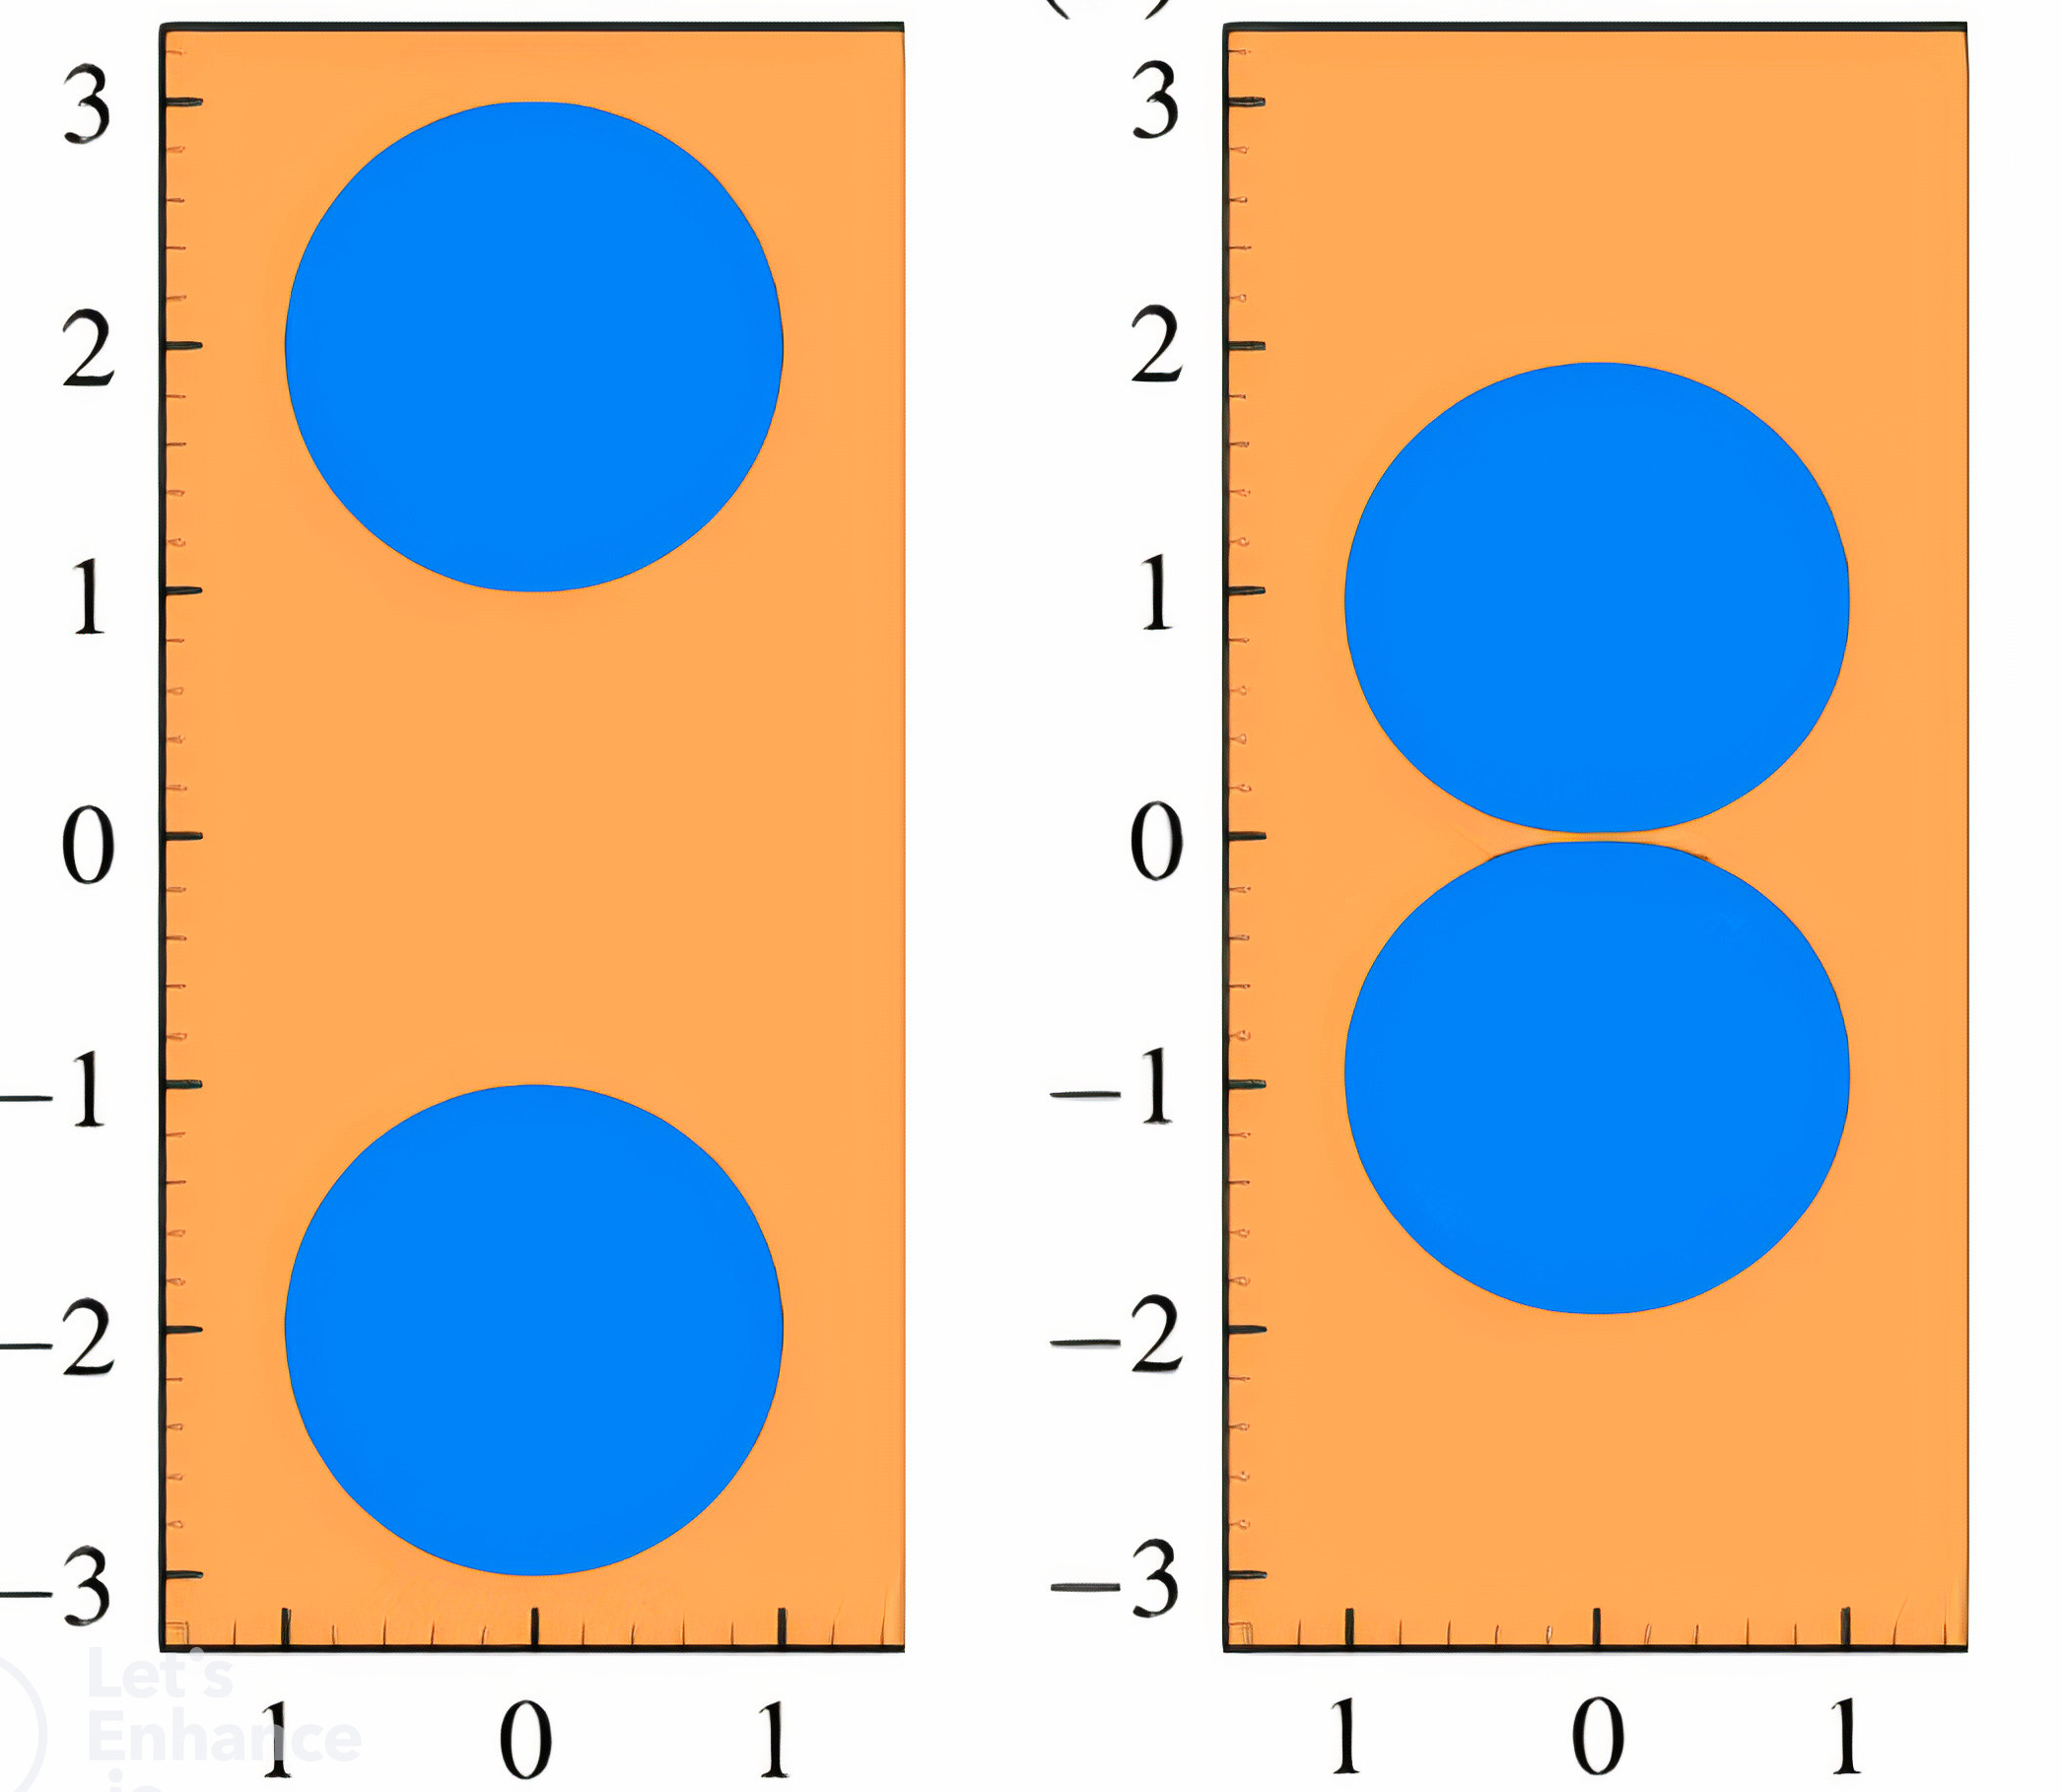
\includegraphics[height=0.22\textwidth]{image/coalesence2.jpg}};
        \node (img2) at (0\textwidth,0\textwidth) {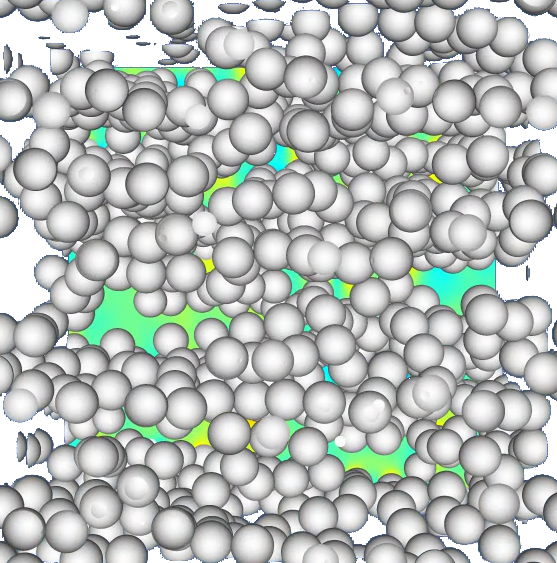
\includegraphics[height=0.25\textwidth]{image/700drop.png}};
        \node[very thick,fill=white,draw=gray] (ttx) at (0\textwidth,0.25\textwidth)
        {
        \begin{minipage}{4.4cm}
            Closure terms:
            \begin{itemize}[topsep=0pt, partopsep=0pt]
                \setlength{\itemsep}{0pt} 
                \setlength{\parskip}{0pt}
                \item \textcolor{red}{Interphase drag force}.
                \item \textcolor{red}{Velocity fluctuation}.
                \item Coalesence kernel.
                \item \ldots
            \end{itemize}
        \end{minipage}
        };
        \node[very thick,fill=white,draw=gray] (ttx2) at (0\textwidth,-0.35\textwidth)
        {
            \begin{minipage}{4.4cm}
                Constrained parameters:
                \begin{itemize}[topsep=0pt, partopsep=0pt]
                    \setlength{\itemsep}{0pt} 
                    \setlength{\parskip}{0pt}
                    \item Volume fractions. 
                    \item Phase density ratio. 
                    \item Phase viscosity ratio. 
                    \item \ldots
                    % \item Frequency of collision. 
                    % \item Interaction forces.
                \end{itemize}
            \end{minipage}
        };
        \node (img3) at (0.35\textwidth,0.25\textwidth) {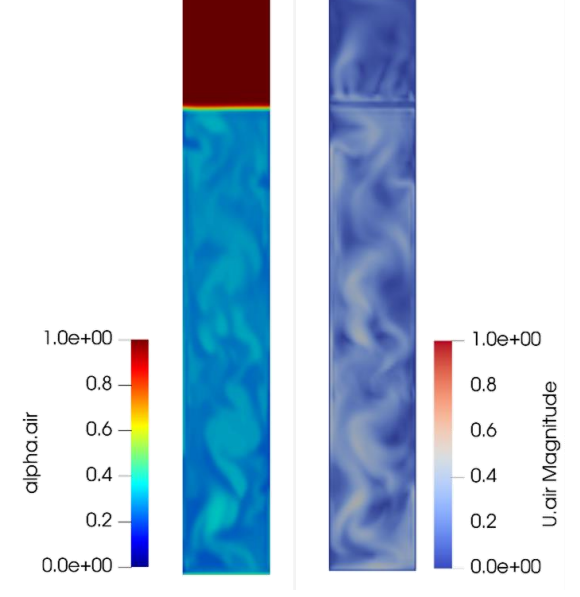
\includegraphics[height=0.25\textwidth]{image/Euler_Euler.png}};
        % \node (img4) at (0.425\textwidth,-0.25\textwidth) {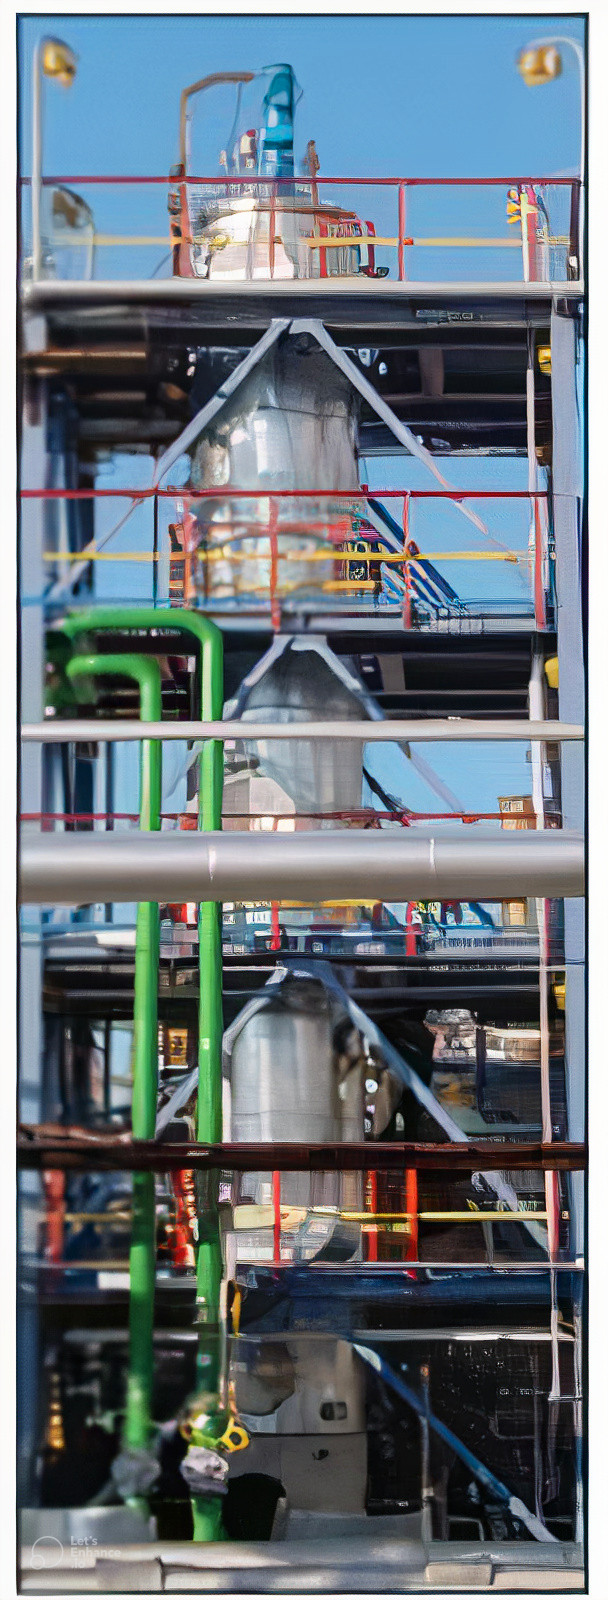
\includegraphics[height=0.25\textwidth]{image/process_LE_auto_x4.jpg}};
        \node (img4) at (0.35\textwidth,-0.25\textwidth) {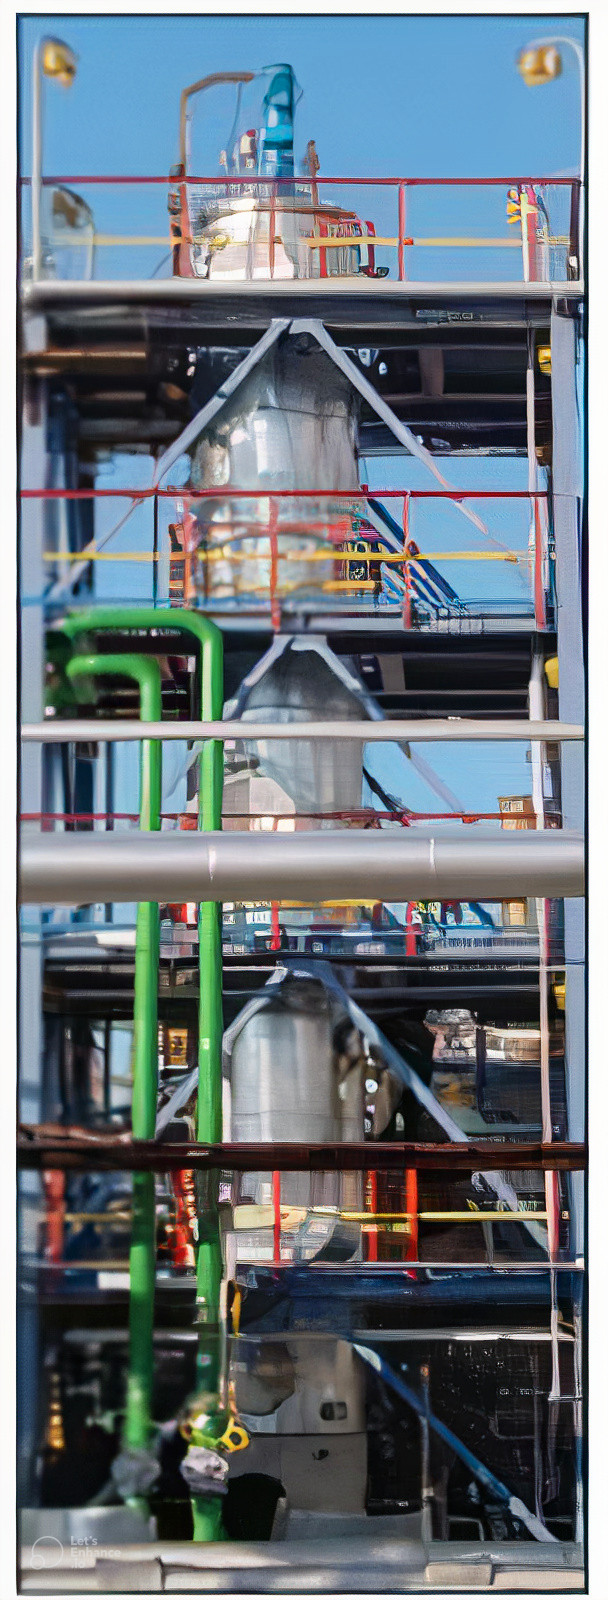
\includegraphics[height=0.25\textwidth]{image/process_LE_auto_x4.jpg}};
        %                   
        %                   
        %                   
        \node[align=center] (imgB) at (-0.35\textwidth,-0.48\textwidth) {\Large \underline{Film scale}};
        \node[align=center] (imgB) at (0,-0.48\textwidth) {\Large \underline{Particle scale}};
        \node[align=center] (imgB) at (0.35\textwidth,-0.48\textwidth) {\Large \underline{Process scale}};
        %
        \node[above,text width=0.3\textwidth] (imgC) at (img1.north) {Direct Numerical Simulation (DNS) \citep{sambath2019inertial}.};
        \node[below,text width=0.3\textwidth] (imgD) at (img2.south) {Particles Resolve Direct Numerical Simulation (PR-DNS).};
        \node[above,text width=0.3\textwidth] (imgC) at (img3.north) {Euler-Euler simulation of the processes. };
        \node[below,text width=0.3\textwidth] (imgC) at (img4.south) {Prototype / final product};
        %
        %
        \draw[->,very thick] (img1) -- (ttx.west);
        \draw[->,very thick] (img3) -- (img4)node[midway,fill=white,draw=gray]{
        \begin{minipage}{4.4cm}
            Optimized:
            \begin{itemize}[topsep=0pt, partopsep=0pt]
                \setlength{\itemsep}{0pt} 
                \setlength{\parskip}{0pt}
                \item Geometry of process. 
                \item Inter-phase transfer.
                % \begin{itemize}[topsep=0pt, partopsep=0pt]
                %     \setlength{\itemsep}{0pt} 
                %     \setlength{\parskip}{0pt}
                %     \item Thermique
                %     \item Chemical
                % \end{itemize}
                \item \ldots
            \end{itemize}
        \end{minipage}
        };
        \draw[->,very thick] (img2.north) -- (ttx);
        \draw[->,very thick] (img2) -| (img1)node[midway,fill=white,draw=gray]{
        \begin{minipage}{4.4cm}
            Constrained parameters:
            \begin{itemize}[topsep=0pt, partopsep=0pt]
                \setlength{\itemsep}{0pt} 
                \setlength{\parskip}{0pt}
                \item \textcolor{red}{Interaction kinematics }  
                \item Frequency of collision. 
                \item Interaction forces.
            \end{itemize}
        \end{minipage}
        };
        \draw[->,very thick] (img4) -- (ttx2);
        \draw[->,very thick] (ttx2) -- (imgD);
        %
        \draw[->,very thick] (ttx.east) -- (img3);
        \draw[red,very thick] (img2.south west) rectangle(img2.north east);
        %
        \draw[very thin, dashed] (current bounding box.north)++(-0.175\textwidth,0) -- (-0.175\textwidth,0);
        \draw[very thin, dashed] (current bounding box.south)++(-0.175\textwidth,0) -- (-0.175\textwidth,0);
        \draw[very thin, dashed] (current bounding box.north)++(0.175\textwidth,0) -- (0.175\textwidth,0);
        \draw[very thin, dashed] (current bounding box.south)++(0.175\textwidth,0) -- (0.175\textwidth,0);
    \end{tikzpicture}
    \caption{Scaling up strategy of the process optimization.  The text in red and the red box represent the topics treated in this PhD. 
    Global description: 
    The process need to be modeled with averaged simulations; the averaged ``Euler-Euler'' simulations needs closures laws; these closure laws are provided by the film scale problem and particles scale problem; Both problem are driven by the parameters given by the upper-scale situation, which is the industrial reactor or process scale. }
    \label{fig:scaling_up}
\end{figure}

As one-to-one sized experiments of the processes are often too expensive to carry out, we aim to conduct numerical simulations based on ``averaged conservation laws'' that are valid at the macroscale. 
Another reason for this choice is the ease of measuring physical quantities that is afforded by numerical simulations, compared to real-life experiments, which often require invasive or inaccurate measurement tools.
Of course, throughout the optimization process, validation with experimental data will be necessary to ensure the reliability and accuracy of the simulation results. 
Note that these ``averaged conservation laws'' require models that account for the physics driving the mesoscale (and microscale) behavior of the flow. 
Thus, this PhD work primarily focuses on deriving the ``averaged conservation laws'' (discussed below) and on providing mesoscale models based on the problem of droplet-droplet interaction with the surrounding fluid.

\subsection{Mathematical modeling of dispersed two-phase flows }

We would now like to briefly present the methodology employed to derive these ``averaged conservation laws'', which will enable us to build numerical simulations of the above processes of interest.
Before doing so we provide a short discussion on kinetic-theory of gases as the method to build averaged equations for dispersed two-phase flows model is partly inspired by this theory. 

Note that multiphase flows can take several forms depending on the topology of the mixture. In this thesis, we focus on dispersed multiphase flows.
In this type of flow, the mixture consists of a continuous dominant phase, with inclusions dispersed within it. These inclusions can be of various natures, such as solid particles, liquid droplets, or gas bubbles.

\subsubsection{Links with the kinetic theory of gases}

We would like to begin our presentation with the smallest scale possible: the scale of the molecules that constitute a fluid or gas.
In a very simplistic approach, at this scale, molecules can be modeled as spheres colliding with each other \citep{kardar2007statistical}. 
The behavior of a single molecule can be described using Newton's second law, which states that the sum of all forces acting on a particle is equal to its mass multiplied by its acceleration, $\sum\textbf{F} = m \textbf{a}$. 
Essentially, this law allows us to predict the trajectory of one or several particles over time. 


To model a fluid or gas, essentially an ensemble of particles colliding with each other, Newton's second law becomes impractical due to the vast number of particles present in a unit volume of liquid or gas.
Thus, instead of modeling all individual particle trajectories, we derive equations for the average particle velocities and trajectories.
This is achieved through statistical methods, particularly the statistical kinetic theory of gases \citep{hansen2013theory,kardar2007statistical}.
For instance, the well-known Boltzmann equation describes the evolution of the one-point probability density function, representing the likelihood of finding a particle at a given location with a specific velocity.
Averaging this equation, multiplied by the velocity vector, leads to the Maxwell equations, which describe the balance of the averaged velocity of particles in a volume of fluid or gas.
These equations can be seen as the momentum balance for a fluid or gas.
It is important to note that they still represent the average velocity of all particles within the fluid.
Through this averaging procedure, fluids or gases, despite being composed of discrete particles, are viewed as continuous media at the microscopic scale.
Then, their specific behavior (Newtonian, non-Newtonian, shear-thinning, elastic, etc.) arises as a consequence of subscale interactions, which are captured through ``constitutive laws'' or ``closure terms''.
In other words, in the averaged equations describing the properties of the fluid, these closure terms represent the subscale physics that is needed to obtain a realistic model of the fluid.
By assuming the fluid is at thermodynamic equilibrium and exhibiting Newtonian behavior, for example, the equations governing fluid motion reduce to the Navier-Stokes equations. 

The main takeaway from this modeling approach is that, due to the vast number of particles in a parcel of fluid, we use probabilistic arguments to compute the averaged properties of the ensemble of particles, treating them as a continuum.
The upscaling strategy for modeling liquid-liquid separation and flotation processes follows a similar principle.
At a scale of approximately $1000$ droplet sizes, the Navier-Stokes equations become computationally expensive to solve numerically.
To address this, we rely on averaged equations that describe the mean motion of the dispersed and continuous phase.
This is referred to as the ``two-fluid'' model, initially developed by \citet{drew1983mathematical}.
In this framework, we require two sets of equations: one set to describe the dispersed phase (droplets or bubbles) and another to describe the motion of the continuous phases.
The parallel with kinetic theory can be extended further, as the centers of mass of the droplets or bubbles obey Newton's second law of motion, similar to the particles that constitute fluids and gases.


Thus, whether we aim to model numerous molecules or droplets, the procedure is essentially the same: we derive conservation laws for the averaged properties of an ensemble of particles (or droplets) rather than predicting the evolution of each individual particle (or droplet).
However, there is a notable difference between the modeling of molecules and two-fluid mixtures, beyond the obvious differences in size and shape between droplets and particles.
Molecules are typically assumed to evolve in a vacuum, interacting only with other molecules, while droplets interact continuously with the surrounding continuous phase and other droplets.
The predominance of droplet-continuous phase interactions over droplet-droplet interactions fundamentally changes the structure of the equations compared to the one governing the fluid at the microscale.
As a result, the methodology for deriving averaged two-phase flow equations differs significantly from that used in the kinetic theory of gases.
Nevertheless, the approach is conceptually similar.
Below, we describe in more detail the strategy employed to derive these averaged equations. 


\subsubsection{From the microscopic to the process scale}

Assuming that the Navier-Stokes equations govern the mesoscale motion in both the continuous and dispersed phases, we can derive the two-fluid averaged Navier-Stokes equations to model the macroscale motion of each phase. 
These averaged equations typically consist of the mass and momentum balance for the dispersed phase and the mass and momentum balance for the continuous phase. 
The unknowns in these equations include, for instance: The averaged velocity of the continuous phase, $\textbf{u}_f$; The averaged velocity of the droplets $\textbf{u}_p$; The volume fractions of the continuous and dispersed phases, $\phi_f$ and $\phi_d$, respectively. 
To be representative, these equations require information about the sub-scales (i.e., the micro- and mesoscale dynamics).
As discussed above, the ``closure terms'' are mathematical expressions present in these averaged equations to account for the influence of subscale physics on the macroscale behavior. 
By ``mesostate'' we refer to the set of parameters describing the local properties of an emulsion at the droplet scale.
This includes:  droplet sizes, droplet shapes, droplet positions, droplet velocities, the velocity and pressure fields of the continuous phase around the droplets\footnote{
    The term ``mesostate'' is inspired by the concept of ``microstate'' commonly used in statistical mechanics, which refers to the instantaneous list of parameters describing the state of a system at the molecular level. Specifically, a microstate includes the molecule positions and velocities at a given moment.
    }. 
As an example, the closure terms can include the averaged drag force between the phases, the local velocity fluctuations, and the averaged Newtonian stress, all of which may be expressed in terms of the macroscopic unknowns ($\textbf{u}_p$, $\phi_d$, and $\textbf{u}_f$) to close the problem.
Consequently, solving these equations numerically requires a precise expression of the closure terms as a function of the macroscopic properties and, of course, an efficient solver to run the macroscale simulation and model the process.

The closure terms depend on what we call the probable ``mesostate'' of the flow. 
However, the existing ``mesostate'' can span an infinite phase space of parameters required to fully describe the local state of the continuous and dispersed phases.
It is clear that deriving an analytical expression of the closure terms valid for all possible ``mesostates'' is too complex.
Therefore, studies are often limited to very specific situations to derive closure terms.
For example, it is often assumed that the dispersed phase consists of spherical particles and that the suspension is monodisperse, meaning all particles in the mixture have the same size.
In these simplified scenarios, some authors have successfully closed the averaged two-fluid Navier-Stokes equations theoretically.
For example, \citet{jackson1997locally} derived an averaged set of equations for a monodisperse suspension of solid spherical particles, where the closure terms were obtained under the assumption that the relative motion between the dispersed and continuous phases follows the Stokes equations. 
Similarly, \citet{zhang1997momentum} developed a set of averaged equations for a mono-disperse emulsion of spherical droplets, with the closure terms derived within the context of Stokes flow as well.


The preceding authors considered monodisperse suspensions; however, another crucial challenge for averaged equations is the modeling of the local size distribution of droplets within a given volume containing the emulsion.
The size distribution can be influenced by the migration of particles that possess different rising velocities due to their size variations, and by coalescence and breakup phenomena, which are governed by mechanical and colloidal interactions.
The modeling of polydisperse flows involves the use of what are called Population Balance Equations (PBE), a related but distinct system of equations than the two-fluid averaged Navier-stokes equations.


To summarize, we have demonstrated that modeling the above processes involves using averaged conservation laws that require ``closure terms''. 
These terms account for the mesostate and microstate behaviors of the emulsion. 
This upscaling methodology avoids the computational expense of directly solving the detailed flow and chemical interactions throughout the entire vessel.
To construct models, one must first study the interactions between multiple droplets and the continuous phase. 
In a second step, it is necessary to examine droplet-droplet interactions to better predict coalescence and breakup phenomena. 


These investigations require a combination of theoretical, numerical, and experimental data. 
The problem of droplet-droplet interactions leading to coalescence (i.e. the film drainage problem) can be addressed either experimentally or by employing Direct Numerical Simulation (DNS)  (see \ref{fig:scaling_up} (left)).
To model the interaction between multiple droplets and the continuous phase, we can use Particle-Resolved Direct Numerical Simulation (PR-DNS) \citep{tryggvason2006direct}, (see \ref{fig:scaling_up} (right)).
This approach is similar to DNS, however, it does not fully resolve the flow within the film between two interacting particles.
Indeed, accurately solving the flow around hundreds of droplets while also resolving the flow within the film during droplet collisions would be computationally too expansive.




\subsubsection{Mathematical formulations}

We would now like to provide a general picture of the different methodologies employed to model dispersed systems, whether it is for two-fluid flows, for granular materials, or (as it is the case in kinetic theory) molecules. 
On \ref{fig:diagram2} we represent these different modeling strategies with a study of reference for each category. 
Firstly, we can identify two main areas on \ref{fig:diagram2}, namely, the ``Lagrangian-'' and ``Eulerian-'' based models. 
The former corresponds to the models that use Lagrangian laws to describe the dispersed phase, and that are then averaged to obtain macroscopic equations. 
In opposition, the ``Eulerian-based models'' use an ``Eulerian'' approach to describe the continuous (and dispersed) phase, and then employ an average procedure to derive the macroscopic equations. 
Our classification identified four main categories, ``Kinetic-Theory'', ``Population-Balance-Models'' (PBE or PBM), ``Euler-Euler Two-fluid models'' (or just ``Two-fluid models''), and finally ``Hybrid models''. 
% \begin{figure}[h!]
%     % \begin{tikzpicture}[thick, scale=0.5]
%     \centering
%     \begin{tikzpicture}[thick, scale=1, every node/.style={scale=0.45}]
%         \node (img) at (0,0){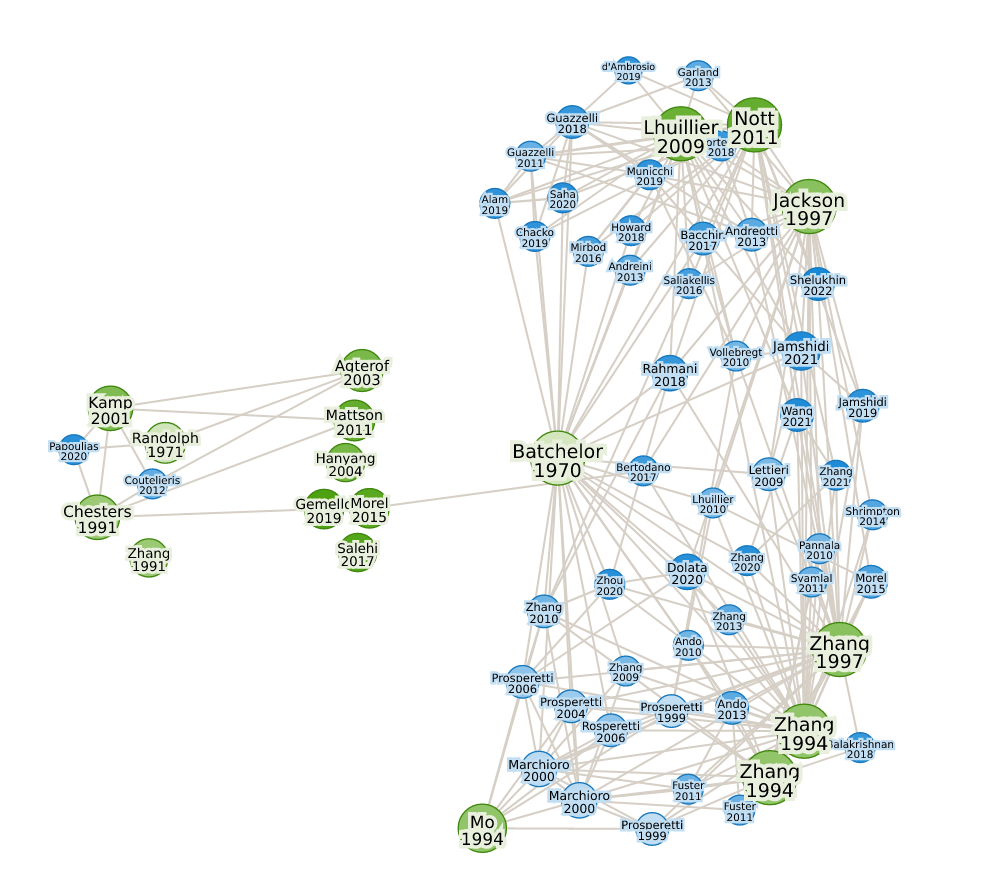
\includegraphics[width=2\textwidth]{Bib/graph70_paperGraph_network.png}};
%         \draw[dashed,very thick](-2,-0.5)ellipse(1 and 2.5);
%         \draw[dashed,very thick](-5,-0.5)ellipse(1.5 and 2.5);
%         \draw[dashed,very thick](4,4)ellipse(2 and 1.5);
%         \draw[dashed,very thick](4.5,-4)ellipse(1.5 and 2);
%         \draw[dashed,very thick](4,5)node[above,very thick]{\Large$\textbf{(III)}$};
%         \draw[dashed,very thick](6,-5)node[right,very thick]{\Large$\textbf{(II)}$};
%         \draw[dashed,very thick](-6.5,2)node[above,very thick]{\Large$\textbf{(I)}$};
%         \draw[dashed,very thick](-1.3,1.75)node[above,very thick]{\Large$\textbf{(IV)}$};
%         % \draw[<->](com2.north)--(com3.south)node[midway]{Equivalent};
%     \end{tikzpicture}
%     \caption{Non-exhaustive cartography of the different publications on population balance models and averaged equations. The articles are represented by the name of the first author. The lines between each article mean that both articles cited each other.}
%     \label{fig:carte}
% \end{figure}
\begin{figure}
    \centering
    \begin{tikzpicture}[node distance=10pt,font=\footnotesize]
    \tikzset{
        venn box/.style={
          draw=black, very thick, 
          rounded corners=10,
          inner xsep=10pt, inner ysep=15pt, outer ysep=5pt
        },
        venn numbers/.style={
      %    draw,
          inner ysep=0pt,
          align=center
        },
        venn title/.style={
          fill=black, text=white
        }
      }            
    \node[venn box,fill=gray!5] (N) {%
        \citet{rao2008introduction}
    };
    \node[venn numbers, above=of N] (Z-N) {
        \citet{marchisio2013computational}
    };
    \node[venn box, fit=(Z-N) (N) ] (Z) {};
    \node[venn numbers, above=of Z, align=center] (Q-Z) {};
    \node[venn box,fill=gray!5] (Q) at (5.5,0) {
        \citet{morel2015mathematical}
    };
    \node[venn numbers, right=of Q, inner sep=0pt, align=center] (Q-two) {
        \citet{drew1983mathematical}
    };
    \node [venn box, fit= (Q) (Q-two)] (R) at (6.5,0) {};
    \node [venn box, fit=(R),gray,dashed,inner ysep=50pt] (El) {};
    \draw[gray] node[fill=white,anchor=north west] at ([shift={(10pt, 3pt)}]El.north west) {Eulerian-based models};
    \node [venn box, fit=(Q) (Z) ,gray!50,dashed] (D) {};
    \draw[gray!50] node[fill=white,anchor=north west] at ([shift={(10pt, 3pt)}]D.north west) {Lagrangian-based models};
    \tikzset{every node/.style=venn title}
    \draw node[anchor=north east] at ([shift={(-10pt, 3pt)}]R.north east) {Two-fluids model};
    \foreach \i/\j/\k in {N/Kinetic-Theory/0, Z/PBE/10pt, Q/Hybrid model/10pt} {
        \draw node[anchor=north west] at ([shift={(10pt, 3pt)}]\i.north west) {\j};
              %node[rounded corners] at ([yshift=-\k]\i.east) {${\i}$};
              }

      \end{tikzpicture}
    \caption{Mathematical modeling of dispersed two phases flows cartography. 
    Lagrangian-based model: corresponds to the averaged model derived by averaging Lagrangian governing laws on each particle constituting the dispersed phase. 
    Eulerian-based model: corresponds to the averaged model derived by averaging the Eulerian governing laws valid within each phase of the flow. }
    \label{fig:diagram2}
\end{figure}


The area denoted by ``Kinetic-Theory'' represents the studies dedicated to the modeling of Gases and liquid \citep{hansen2013theory,kardar2007statistical}, however  
``Kinetic-Theory'' can also be used to describe elongated particles \citet{curtiss1956kinetic}, which is useful to model material constituted with orientable structures of molecules.
It can also be used to describe more macroscopic phenomena such as granular materials \citet{rao2008introduction}.  
Extending this theory to poly-disperse assemblies of particles one obtains the so-called PBE. 
The only aspect that changes is that PBE includes equations to be solved for the probability distribution of the particle size, or the moments of that distribution \citep{fox2023generalized,randolph2012theory}. 
The former two modeling approaches focused mainly on the modeling of the dispersed phase.
The continuous phase (when there is one) is treated by averaging the Eulerian conservation laws of the fluid. 
However, the mathematical relation between the dispersed phase and continuous phase is made somewhat empirically since the equations of both phases are derived independently. 
That is the reason why the ``Kinetic-Theory'' and PBE models are not included in the ``Eulerian-based'' models. 

Let us focus on a liquid-liquid system such as an emulsion. 
In this case, the majority of averaged two-fluid models are based on the framework proposed by \citet{drew1983mathematical}, where the equations for both the dispersed and continuous phases are derived by averaging the local Eulerian conservation laws governing the fluid in each phase.
Despite its versatility allowing applications beyond dispersed flows, such as stratified or slug flow, the physical interpretation of the closure terms remains difficult \citep{drew1983mathematical}.
Additionally, the droplet-size distribution (which is highly relevant for the industrial processes mentioned above) cannot be determined with these models, because by definition ``Two-fluids models'' do not assume that one of the phase is dispersed within the other.
Nevertheless, one advantage of this model compared to PBE or ``Kinetic-Theory'', is that the terms of exchanges between phases are consistent. 
Meaning that we recover the exact same terms in the equations of the dispersed phase and in the equation of the continuous phase. 

Consequently, to model emulsions, we need a model  which is able to describe the topology of the flow, such as the size distribution of droplets, their deformation and so on, and that is properly linked with the continuous phase, so that the global set of equations remains consistent. 
Such a model is termed ``Hybrid model'' since it is a Lagrangian- / Eulerian- based model.
The difference with the previous models is that the Eulerian-based exchange terms in the continuous phase equations are termed into Lagrangian-based exchange terms, which correspond exactly to the exchange terms appearing in the Lagrangian-based equations describing the dispersed phase. 

Many previous studies that used the ``hybrid'' formalism have focused on solid particles \citep{buyevich1979flow,jackson1997locally}. 
Notable exceptions include \citet{zhang1994ensemble}, who investigated spherical bubbles with time-varying radii, and \citet{zhang1997momentum}, who examined spherical droplets. 
Despite these advances, the question remains: how can different inclusion shapes, internal fluid motion, and surface transport equations be incorporated into such Lagrangian models? 
To the best of our knowledge, important surface properties, such as variable or constant surface tension, the arbitrary shape of fluid particles, and the distribution of surfactants, have not yet been fully incorporated into current averaged ``hybrid models''.  
A good review of the ``hybrid model'' for bubbly flows can be found in \citet{paisant2014modelisation,morel2015mathematical}. 

Overall a model relating kinetic-theory-like equations while taking into account the fluid nature of the droplets seems absent from the literature. 
In this manuscript, we propose a general framework able to describe a dispersed phase of arbitrary nature with surface properties while being consistent with the kinetic-theory-like model.

\subsection{The closure problem}

Either it is for PBE, Kinetic-Theory, Two-fluid or Hybrid  models, one needs accurate closure terms. 
In this work, we classified the closure terms into three groups. 


\subsubsection{First group}
The first group represents the closure terms that are common to any dispersed phase type. 
For example, the drag force term, the Reynolds stress (or pseudo-turbulent stress), and the first moment of force term, appear in every averaged model, regardless of the dispersed phase nature (solid particles, bubbles, or droplets \ldots). 
Hence, numerous studies have already developed models for these closures. 

In our configuration, a drag force correlation should predict the mean drag force density as a function of the local \textit{Reynolds} number based on the particle size, denoted as $Re$, and the volume fraction of the dispersed phase, $\phi$. 
Additionally, since we are considering droplets with a constant density ratio ($\zeta$) but arbitrary viscosity, the model must account for the viscosity ratio, $\lambda$. 
Countless studies have been conducted to develop accurate drag force models. 
\citet{schiller1933} and \citet{mei1994} developed a drag force model for isolated solid spherical particles and isolated spherical bubbles, respectively.
Based on these two coefficients \citet{magnaudet1997forces} proposed a drag force model accounting for arbitrary viscosity ratio $\lambda$ and $Re$, for isolated spherical droplets. 
To take into account the volume fraction of droplets into the drag coefficient it is customary to multiply the ``isolated'' drag coefficient by a ``swarm factor''. 
A large number of studies have been devoted to build ``swarm factors'' for solid particle and bubble suspensions. % \citep{simonin2016drag,tenneti2011drag,chen2023review}.
Reviews, discussions, and benchmarks can be found in \citet{simonin2016drag,tenneti2011drag,chen2023review}. 
However, fewer studies on ``swarm factors'' in droplets suspensions can be found in the literature. 
The theoretical analysis of \citet{wacholder1973,haber1981} although providing a drag force correlation for sedimenting assembly of spherical droplets (valid for arbitrary $\lambda$), is limited to $\phi \ll 1$ (but non-zero) and $Re =0$. 
The pioneering study of \citet{richardson1954} proposed to model the ``swarm factor'' using the formulation:  $(1-\phi)^n$, where $n$ is an empirical constant.  
\citet{ishii1979drag} by compiling various experiments found in the literature proposed values for this coefficient adapted to droplets suspensions, hence providing a drag force coefficient valid for arbitrary $\phi$ and $\lambda\approx 1$.
Nevertheless, no existing model in the literature comprehensively describes the dependence of drag force density in terms of $Re$, $\phi$, and arbitrary $\lambda$. 

Reynolds stress\footnote{The Reynolds stress is a second-order tensor that represents the variance of the local continuous phase velocity in each direction of space.}  models are far less frequently proposed in the literature. 
In the first place, theoretical analysis have been conducted by \citet{biesheuvel1984two} considering particles immersed in potential flows ($Re\to\infty$), and in the dilute regime ($\phi=0$). 
Then, based on DNS and experiments \citet{mehrabadi2015pseudo,almeras2021statistics},  and \citet{xia2022improved} proposed different models for the Reynolds stress tensor, all focusing on suspension of solid spherical particles. 
Even though their models span a wide range of $Re$ and $\phi$ (sufficient for our applications) it still misses the $\lambda$ dependency. 
However, a Reynolds stress model that accounts for arbitrary $\lambda$ could not be found in the literature. 

The averaged first moment of force (also called the Stresslet) is another closure term of interest.
In the Stokes and dilute regimes this term is the cause of the ``Einstein-equivalent viscosity''  of a suspension \citep{guazzelli2011}, it is therefore crucial for the modeling of dispersed two-phase flows. 
For droplets or deformable droplets \citet{rallison1978note} and \citet{nadim1996concise} derived closure for the Stresslet term in the Stokes flow regime.  
At non-vanishing inertial effect \citet{raja2010inertial} determined the first order correction in Reynolds number of the Stresslet. 
In \citet{batchelor1972hydrodynamic} and in \citet{hinch1977averaged}, they derive an expression for the Stresslet for suspensions made of solid spherical particles accurate at $\mathcal{O}(\phi^2)$.
These studies all considered neutrally buoyant, droplet or solid particle suspensions, i.e. with no relative motions between the dispersed and continuous phases. 
However, no study could be found regarding the modeling of the averaged Stresslet in the context of non-neutrally buoyant suspensions. %, or non-dilute suspensions of droplets. 

\subsubsection{Second group}

The second group corresponds to the closure terms that appear solely because the dispersed phase is made of fluid inclusions. 
This includes the droplets internal kinetic energy, the droplets internal viscous dissipation, and so on. 
% For example the internal viscous dissipation within the droplets is a closure term.
These terms appear in the equations only because we will consider an ``hybrid'' formulation of the averaged equations, and because the dispersed phase is made of fluid particles. 
As mentioned above, the ``hybrid'' formulations dealing with fluid particles are not common. 
Hence, these closure terms are rarely studied. 
Thus, a clear lack of understanding to model these terms is present.  

\subsubsection{Third group}

The third and final group is the PBE-related closure terms. 
These include the coalescence and break-up kernels that act as source terms in the size-distribution equation. 
There is an extensive body of literature on coalescence. 
A review of this literature can be found in the works of \citet{chesters1991modelling}. 
However, due to the multi-physics and multi-scale nature of the problem, there is currently no predictive model that has achieved consensus in the literature \citep{liao2010literature}. 
Thus, even if enormous efforts have been devoted to the development of these kernels, major advancements still remain to be made. 



\section{Ambition and objectives of this PhD.}




As the complete problem constitutes an enormous task this PhD focuses on three main aspects: 
(1) The mathematical modeling of dispersed two-phase flow, this includes the development of ``hybrid models'' adapted to the modeling of emulsions, 
(2) the derivation of closure terms in the limit of dilute and Stokes flows regimes,  
and (3) the numerical modeling of the Particle Resolve Direct-Numerical Simulations (PR-DNS) to feed this ``hybrid model'' and extend the domain of validity of the closure terms. 
Despite the use of PR-DNS note that the closure terms developed in this study are still restricted to mono-disperse stead-state buoyant emulsions. 

Additionally, in this work we study only the momentum and mechanical energy equations and related closure terms. 
Meaning that we will not dive into the chemical aspect of the problem. % that is needed to model the liquid-liquid extraction processes. 
We also restrict the study to the particle-scale modeling, hence we will not treat the film-drainage problem and its modeling.   
Nevertheless, we still provide indispensable information regarding the ``Constrained'' or ``input'' parameters that are useful for the film drainage problem. 

In \ref{fig:scaling_up} we present a diagram that summarizes the whole modeling strategy adopted in this PhD work. 
The text and the box colored in red represent the topics treated in this manuscript. 


\section{Outline of the manuscript}


We partitioned this manuscript into three parts. 
% The first one provides a consistent methodology to derive averaged equations, the second part proposes closure models for the averaged equations, and the last part focuses on the droplet-droplet interactions. 

\ref{part:one} focuses on the derivation of the averaged equations as well as the derivation of the closure problem. 
\ref{chap:daniel1} provides a derivation of the averaged equations governing the motion of a dispersed two-phase flow with interfacial transport. 
In \ref{chap:daniel15} we consider emulsions made of Newtonian droplets immersed in a Newtonian fluid and derive the mass, momentum, and energy conservation laws for each phase. 
\ref{chap:deformable} specifically focuses on the modeling of rising spheroidal droplets. 
In \ref{chap:daniel2} we demonstrate how to re-formulate the closure terms of the ``hybrid'' model into \textit{single-particle} conditionally averaged terms. 
We then demonstrate how to derive the corresponding conditionally averaged equations to obtain these terms. 



In \ref{part:two} we propose closure models for the averaged equations of the ``hybrid'' model. 
\ref{chap:DNS} introduces PR-DNS of buoyant emulsions in tri-periodic domains. 
These simulations are conducted using the open source library \texttt{Basilisk C}.
In \ref{chap:closure-disperse} we derive closure laws by solving the conditionally averaged equations in the dilute and Stokes flow limit. 
\ref{chap:mono-disperse,chap:pseudoturbulence} address the issues of modeling the interphase drag force and the Reynolds stress terms, respectively. 
Based on the theory and simulation results we build models taking into account arbitrary $\lambda$, $Re$ ($< 100$), and $\phi$ ($< 0.2$). 



% \paragraph*{Part III:} 
\ref{part:three} focuses on the study of the droplet-droplet interactions. 
In \ref{chap:microstructure} we characterize the droplet relative positions, which we refer to as the study of the microstructure of the emulsion. 
Then, in \ref{chap:microstructure_kin} we study the relative velocity between droplets, i.e. the kinematics of the microstructure. 


We conclude this manuscript with a chapter summarizing the main conclusions and perspectives drawn from the above studies. 